%%%%%%%%%%%%%%%%%%%%%%%%%%%%%%%%%%%%%%%%%
% Beamer Presentation
% LaTeX Template
% Version 1.0 (10/11/12)
%
% This template has been downloaded from:
% http://www.LaTeXTemplates.com
%
% License:
% CC BY-NC-SA 3.0 (http://creativecommons.org/licenses/by-nc-sa/3.0/)
%
%%%%%%%%%%%%%%%%%%%%%%%%%%%%%%%%%%%%%%%%%

%----------------------------------------------------------------------------------------
%	PACKAGES AND THEMES
%----------------------------------------------------------------------------------------

\documentclass[aspectratio=43,serif]{beamer}

\mode<presentation> {

% The Beamer class comes with a number of default slide themes
% which change the colors and layouts of slides. Below this is a list
% of all the themes, uncomment each in turn to see what they look like.

%\usetheme{default}
%\usetheme{AnnArbor}
%\usetheme{Antibes}
%\usetheme{Bergen}
%\usetheme{Berkeley}
%\usetheme{Berlin}
%\usetheme{Boadilla}
%\usetheme{CambridgeUS}
%\usetheme{Copenhagen}
%\usetheme{Darmstadt}
%\usetheme{Dresden}
%\usetheme{Frankfurt}
%\usetheme{Goettingen}
%\usetheme{Hannover}
%\usetheme{Ilmenau}
%\usetheme{JuanLesPins}
%\usetheme{Luebeck}
%\usetheme{Madrid}
%\usetheme{Malmoe}
%\usetheme{Marburg}
%\usetheme{Montpellier}
\usetheme{metropolis}
%\usetheme{PaloAlto}
%\usetheme{Pittsburgh}
%\usetheme{Rochester}
%\usetheme{Singapore}
%\usetheme{Szeged}
%\usetheme{Warsaw}

% As well as themes, the Beamer class has a number of color themes
% for any slide theme. Uncomment each of these in turn to see how it
% changes the colors of your current slide theme.

%\usecolortheme{albatross}
%\usecolortheme{beaver}
%\usecolortheme{beetle}
%\usecolortheme{crane}
%\usecolortheme{dolphin}
%\usecolortheme{dove}
%\usecolortheme{fly}
%\usecolortheme{lily}
%\usecolortheme{orchid}
%\usecolortheme{rose}
%\usecolortheme{seagull}
%\usecolortheme{seahorse}
%\usecolortheme{whale}
%\usecolortheme{wolverine}

%\setbeamertemplate{footline} % To remove the footer line in all slides uncomment this line
%\setbeamertemplate{footline}[page number] % To replace the footer line in all slides with a simple slide count uncomment this line

\setbeamertemplate{navigation symbols}{} % To remove the navigation symbols from the bottom of all slides uncomment this line
}

\usepackage{graphicx} % Allows including images
\usepackage{booktabs} % Allows the use of \toprule, \midrule and \bottomrule in tables
\usepackage[utf8]{inputenc}
\usepackage[czech]{babel}
%\usepackage[T1]{fontenc}
%\usepackage{amsmath}
%\usepackage{amsfonts}
%\usepackage{amssymb}
%\usepackage{amsthm}
\usepackage{graphicx}
\usepackage{array}
\usepackage{mathrsfs}

%\usepackage{cmbright}
\usepackage{pxfonts}
%\usepackage{eulervm}%greek fonts in beamer
%\usepackage{arevmath}%greek fonts in beamer

\usepackage{animate}
\usepackage{movie15}

\newtheorem{definice}{Definice}
\newtheorem{veta}{Věta}
\newtheorem{dukaz}{Důkaz}

\newcommand{\Cbb}{\mathbb{C}}
\newcommand{\Rbb}{\mathbb{R}}
\newcommand{\Zbb}{\mathbb{Z}}
\newcommand{\Nbb}{\mathbb{N}}


\newcommand{\D}[1]{\ensuremath{\operatorname{d}\!{#1}}}
\newcommand{\dif}[3][]{\frac{\D{{}^{#1}#2}}{\D{#3}^{#1}}}
\newcommand{\pardif}[3][]{\frac{\partial^{#1}{#2}}{\partial{#3}^{#1}}}
\newcommand{\pardift}[3]{\left(\pardif{#1}{#2}\right)_{#3}}
\newcommand{\op}[1]{\ensuremath{\hat{\mathbf{#1}}}}
\newcommand{\mat}[1]{\ensuremath{\ifnum\pdfstrcmp{#1}{1}=0 \mathbb{1}\else \mathbf{#1}\fi}}
\newcommand{\bra}[1]{\langle #1 \vert}
\newcommand{\ket}[1]{\vert #1 \rangle}
\newcommand{\bralr}[1]{\langle #1 \vert}
\newcommand{\ketlr}[1]{\vert #1 \rangle}
\newcommand{\braketlr}[2]{\left\langle\left. #1\right\vert #2\right\rangle}
\newcommand{\braket}[2]{\langle #1\vert #2\rangle}
\DeclareMathOperator{\tr}{\operatorname{tr}}
\newcommand{\abs}[1]{{\left\vert #1\right\vert}}
\newcommand{\mean}[1]{{\left\langle #1\right\rangle}}
\newcommand{\un}[1]{\,\mathrm{#1}}
\newcommand{\me}{\mathrm{e}}
\newcommand{\mi}{\mathrm{i}}
\newcommand{\lp}{\left(}
\newcommand{\rp}{\right)}
\newcommand{\at}[2]{\left. #1 \right\vert_{#2}}




%----------------------------------------------------------------------------------------
%	TITLE PAGE
%----------------------------------------------------------------------------------------

\title[Classical string motion]{Classical string motion} % The short title appears at the bottom of every slide, the full title is only on the title page

\author{Vojtěch Liška} % Your name
\institute[PřF MUNI] % Your institution as it will appear on the bottom of every slide, may be shorthand to save space
{
Masaryk University, Faculty of Science \\ % Your institution for the title page
\medskip
\tiny{Supervisor: prof. Rikard von Unge}
%\textit{john@smith.com} % Your email address
}
\date{\today} % Date, can be changed to a custom date

\begin{document}

\begin{frame}[plain]
	\titlepage % Print the title page as the first slide
\end{frame}

%\begin{frame}
%	\frametitle{Přehled} % Table of contents slide, comment this block out to remove it
%	\tableofcontents % Throughout your presentation, if you choose to use \section{} and \subsection{} commands, these will automatically be printed on this slide as an overview of your presentation
%\end{frame}

%----------------------------------------------------------------------------------------
%	PRESENTATION SLIDES
%----------------------------------------------------------------------------------------

%------------------------------------------------
%\section{Multimode optical fibre} % Sections can be created in order to organize your presentation into discrete blocks, all sections and subsections are automatically printed in the table of contents as an overview of the talk
%------------------------------------------------

%\subsection{Subsection Example} % A subsection can be created just before a set of slides with a common theme to further break down your presentation into chunks
%\section{Introduction to propagation in optical fibres}



\begin{frame}
	\frametitle{Objectives}
	\begin{itemize}
		\item Find explicit solutions of classical strings and membranes in various spacetimes, for example:
		\begin{itemize}
			\item expanding universe - de Sitter spacetime
			\item gravitational wave background
			\item interaction with gravitational wave pulse
			\item in proximity of black hole or massive star
		\end{itemize}
	\end{itemize}

\end{frame}



\begin{frame}
	\frametitle{Strings vs particles}
	\begin{table}
		\center
		\begin{tabular}{c@{\hspace{3em}}c@{\hspace{3em}}c}
			particle & open string & closed string
		\end{tabular}
	\end{table}
	\begin{center}
		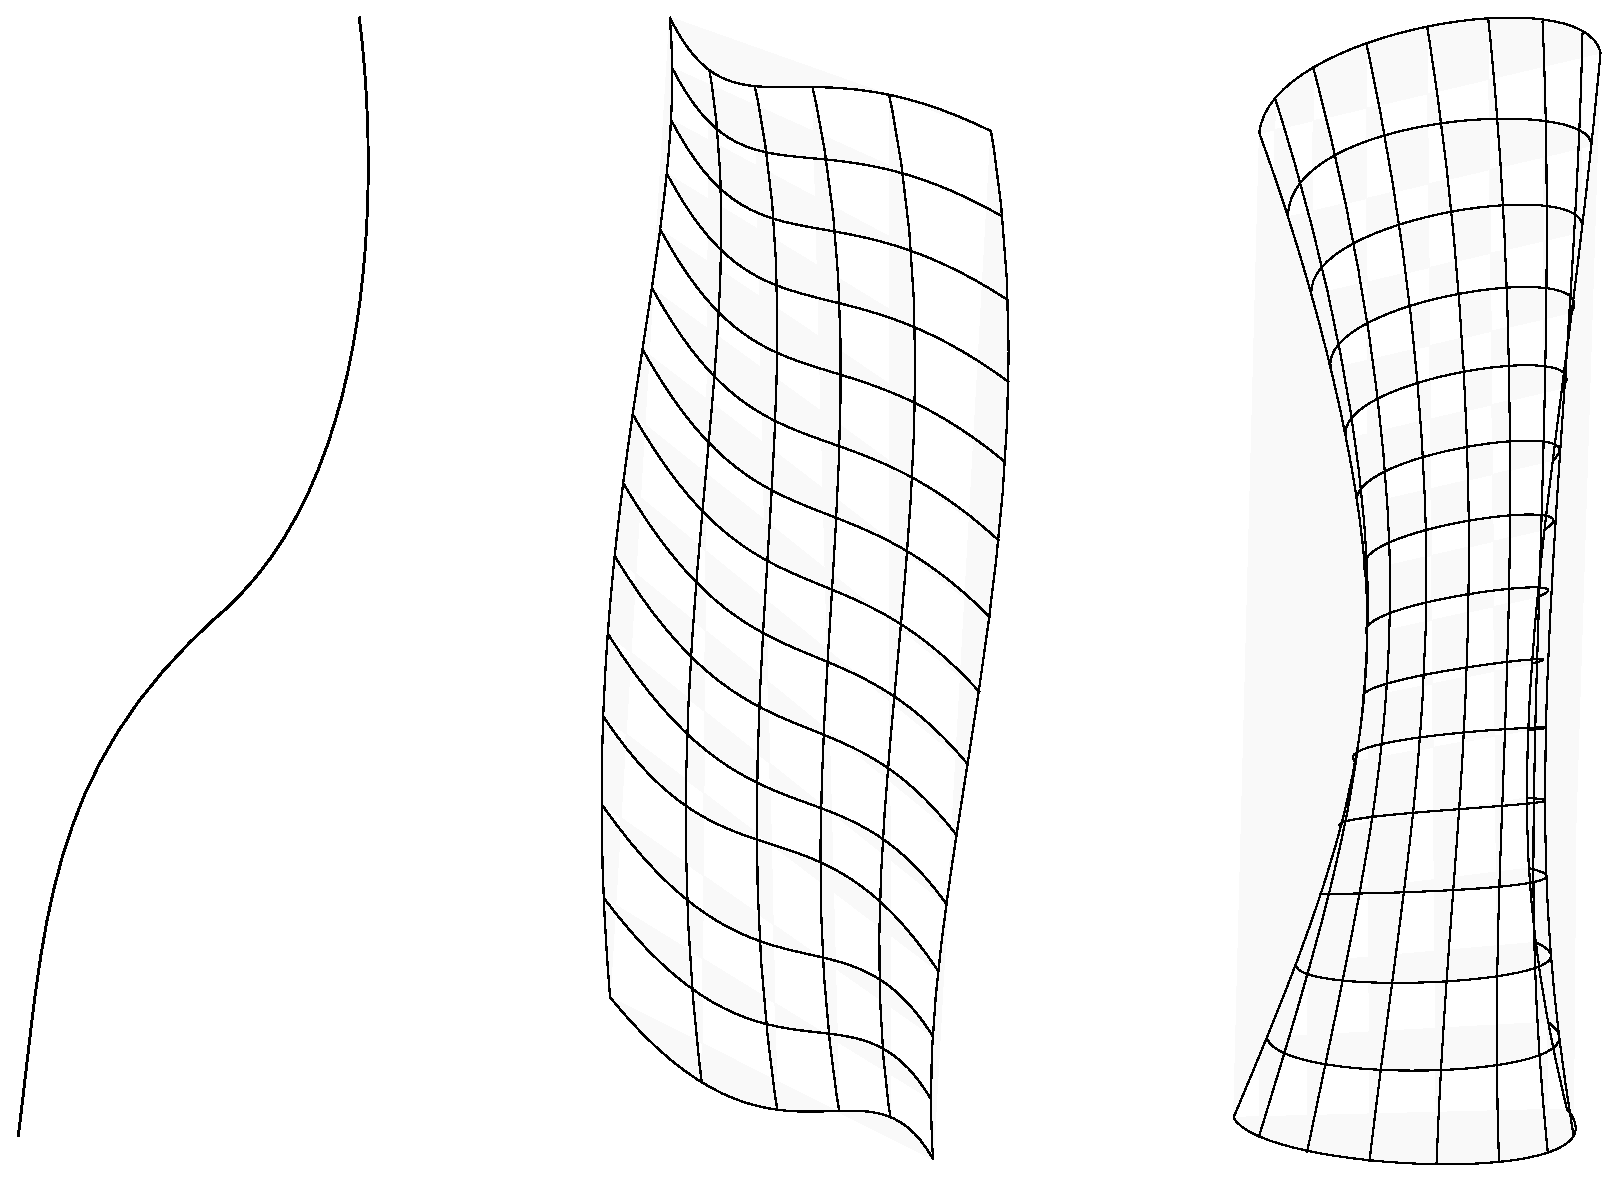
\includegraphics[width=0.7\textwidth]{worldsheet.eps}
	\end{center}
\end{frame}



\begin{frame}
	\frametitle{Nambu - Goto action for strings}
	\begin{itemize}
		\item Action in terms of induced metric on string worldsheet:
		$$		
			S = -T \iint \D \sigma \D \tau \sqrt{-|\gamma|} = -T \iint \D \sigma \D \tau \sqrt{\gamma_{\sigma \tau} 				\gamma_{\tau \sigma} - \gamma_{\tau \tau} \gamma_{\sigma \sigma}}
		$$
		where $\tau$ and $\sigma$ are parametric coordinates on worldsheet.
		\item $\gamma$ in spacetime coordinates $X$:
		$$
			\gamma_{\alpha \beta} = \partial_{\alpha} X^{\mu} ~ \partial_{\beta} X^{\nu} ~ g_{\mu \nu}
		$$
		\item Variation gives:
		$$
		\begin{aligned}
		\delta S = T \iint \D \sigma \D \tau \left[ \partial_{\alpha} \lp \sqrt{-|\gamma|} ~ \gamma^{\alpha 				\beta} \partial_{\beta} X^{\nu} g_{\mu \nu} \rp - \right. \\
		\left. \sqrt{-|\gamma|} ~ \gamma^{\alpha \beta} \partial_{\alpha} X^{\epsilon} \partial_{\beta} X^{\rho} 				\partial_{\mu} g_{\epsilon \rho}  \right] \delta X^{\mu}
		\end{aligned}
		$$
		\end{itemize}
\end{frame}


\begin{frame}
	\frametitle{Gauge choice}
	\begin{itemize}
		\item Choosing gauge / parametrisation to simplify equations of motion.
		\item Tricky because we can get trivial solutions.
	\end{itemize}

\end{frame}


\begin{frame}
	\frametitle{Flat spacetime}
	\begin{itemize}
		\item Minkowski metric - with the right gauge choice equations of motion become wave equation:
		$$
		\dif[2] {X^{\mu}} {\tau} - \dif[2] {X^{\mu}} {\sigma} = 0
		$$
		\item Solution are of the form:
		$$
		X^{\mu} = F^{\mu}(\sigma+\tau) + G^{\mu}(\sigma - \tau)
		$$
		with parametrisation conditions:
		$$
		\lp \dif {\vec{X}} \sigma \rp^2 + \lp \dif {\vec{X}} \tau \rp^2 = 1  \qquad \dif {\vec{X}} \sigma \cdot \dif {\vec{X}} \tau = 0
		$$
	\end{itemize}
\end{frame}



\begin{frame}
	\frametitle{De Sitter spacetime}
	\begin{itemize}
		\item Metric of the form:
		$$		
		\D s^2 = -\D t^2 + e^{2Ht} \lp \D x^2 + \D y^2 + \D z^2 \rp
		$$
		where $H$ is Hubble expansion rate.
		
		\item Equations of motion:
		$$
		\dif[2] R t = \frac{1}{R} \left[ \lp \dif R t \rp^2 - 1 + 2HR \lp \dif R t - HR \rp^3 - 3HR \lp \dif R t - HR \rp \right]
		$$
		\item Singularity at $R = 0$. 
		\item In this case Hamiltonian is constant. We can get simpler solution:
		$$
		\dif R t = \frac{R^5 - R^3 + E^2 R \pm \sqrt{E^2 R^4 + E^4 - E^2 R^2}}{E^2 + R^4}
		$$
	\end{itemize}
\end{frame}



\begin{frame}
	\frametitle{De Sitter background}
	\begin{center}
		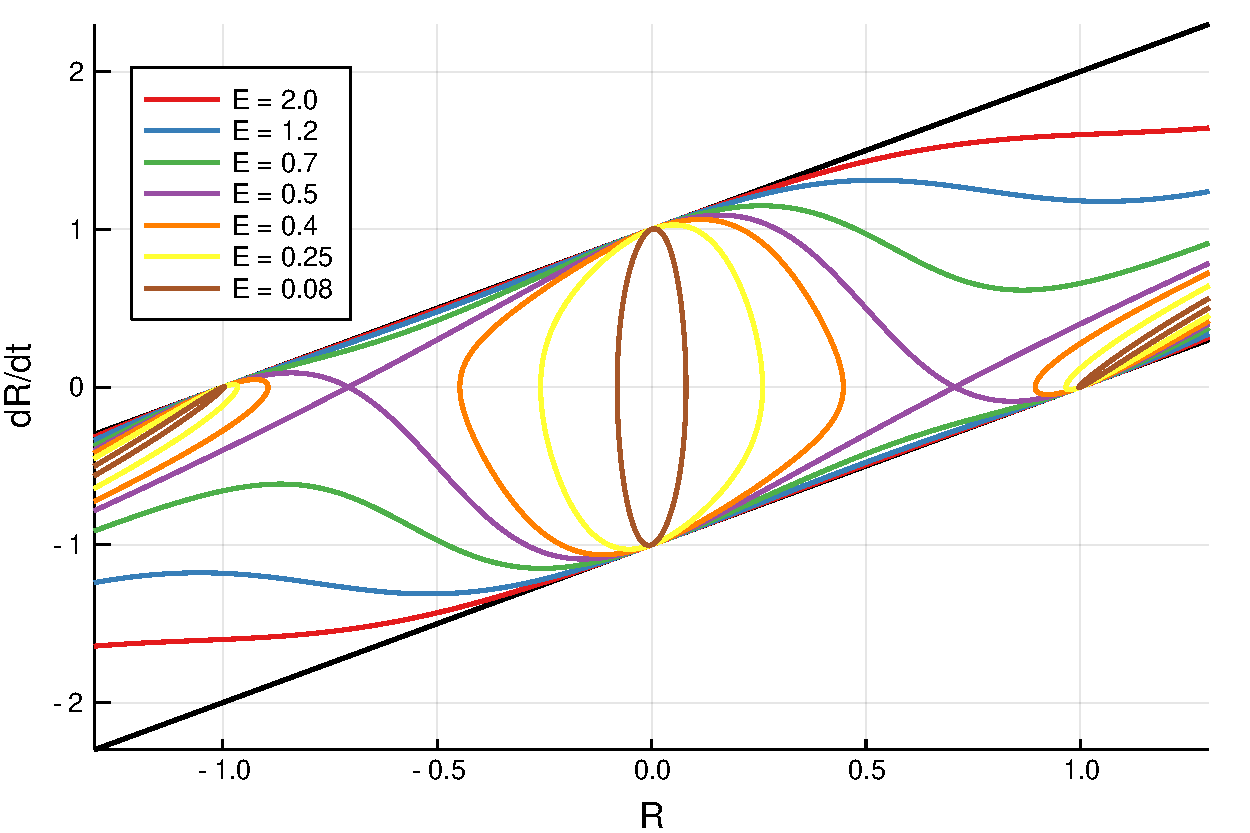
\includegraphics[width=1\textwidth]{DeSitter.pdf}
	\end{center}
\end{frame}

\begin{frame}
	\frametitle{De Sitter background}
	\begin{center}
		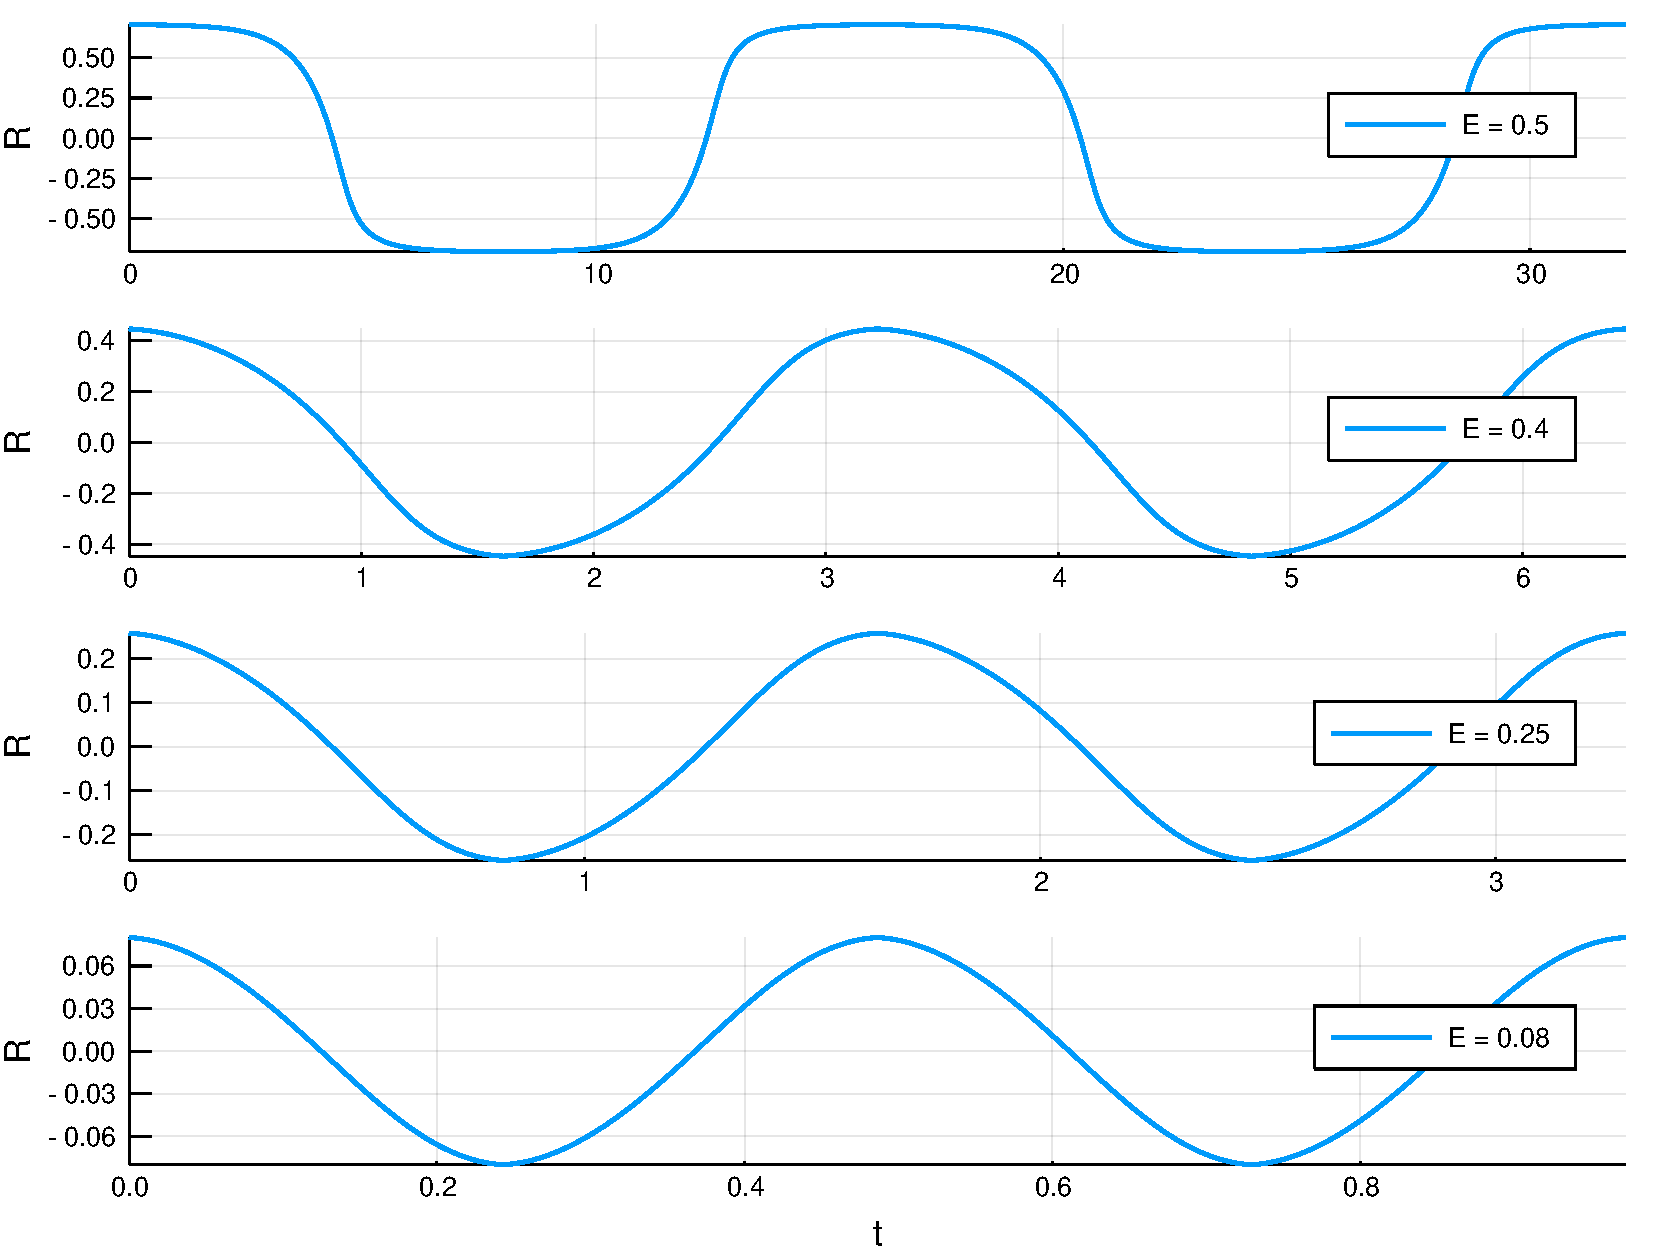
\includegraphics[width=1\textwidth]{Time_dep.pdf}
	\end{center}
\end{frame}

\begin{frame}
	\frametitle{De Sitter background}
	\begin{center}
	\begin{table}
		\center
		\begin{tabular}{c@{\hspace{3em}}c}
			\quad flat spacetime & \qquad de Sitter spacetime
		\end{tabular}
	\end{table}
  	\animategraphics[loop,scale=0.14]{25}{string_flat/string_flat_}{1}{150} \quad \animategraphics[loop,scale=0.14]{25}{string_desitter/string_desitter_}{1}{150}
  	\end{center}
\end{frame}



\begin{frame}
	\frametitle{Gravitational wave background}
	\begin{itemize}
		\item Metric of the form:
		$$
		\D s^2 = H \D U^2 + 2 \D U \D V + \D x^2 + \D y^2
		$$
		where $U = 1/\sqrt{2}(z-t)$ and $V = 1/\sqrt{2}(z+t)$
		\item $H = H(U, x, y)$ satisfies
		$$
		\dif[2] H x + \dif[2] H y = 0
		$$
		\item Equations of motion:
		\begin{gather*}
		\lp \partial_{\tau}^2 - \partial_{\sigma}^2 \rp U = 0 \\
		\begin{aligned}		
		\lp \partial_{\tau}^2 - \partial_{\sigma}^2 \rp V + \partial_U H /2 \left[ \lp \partial_{\tau} U \rp^2 - \lp \partial_{\sigma} U \rp^2 \right] \\
		- \partial_{i} H \left[ \partial_{\tau} U \partial_{\tau} {X^i} - \partial_{\sigma} U \partial_{\sigma} {X^i}\right] = 0
		\end{aligned} \\
		\lp \partial_{\tau}^2 - \partial_{\sigma}^2 \rp X_i - \partial_i H /2 \left[ \lp \partial_{\tau} U \rp^2 - \lp \partial_{\sigma} U \rp^2 \right] = 0
		\end{gather*}
		\item We found possible gauge $U = P^U\tau /T$.
	\end{itemize}
\end{frame}



\begin{frame}
	\frametitle{Summary}
	\begin{itemize}
		\item What I have so far:
		\begin{itemize}
			\item Solution of string motion in flat spacetime.
			\item Radial solution in de Sitter background.
			\item Understanding of gauge choice and some tricks to simplify equations.
		\end{itemize}
		\item In progress:
		\begin{itemize}
			\item Motion in gravitational wave background.
			\item Behavior after interacting with gravitational wave pulse.
			\item Motion close to black hole or massive star.
		\end{itemize}
	\end{itemize}
\end{frame}


%\begin{frame}
%	\frametitle{Vlnová optika}
%	\begin{itemize}
%		\item Vychází z Maxwellových rovnic
%		\item Ve stacionárním případě se řídí Helmholtzovou rovnicí
%		$$
%		\lp \nabla^2 + k^2 \rp \psi \lp\vec{r}\rp = 0
%		$$
%		\pause
%		\item Při separaci proměnných v kartézských souřadnicích vede na řešení ve tvaru rovinných vln
%		$$
%		\psi_k \lp\vec{r}\rp = A e^{i \vec{k} \vec{r}}
%		$$
%	\end{itemize}
%\end{frame}
%
%\begin{frame}
%	\frametitle{Difrakční řešení}
%	\begin{itemize}
%		\item Vývoj světla mezi dvěma rovinami lze vyjádřit propagátorem $\mathcal{H}_{\Delta z}$ v $k$-prostoru
%		$$
%		\psi(z+\Delta z) = \mathscr{F}^{-1} \left\{ \mathscr{F} \{\psi(z)\} \cdot \mathcal{H}_{\Delta z} \right\}
%		$$
%		\pause
%		\item Railegh-Sommerfeldovův propagátor
%		$$
%		\mathcal{H}_{\Delta z}(k_x,k_y)=\text{e}^{\text{i} \Delta z \sqrt{k^2-k_x^2-k_y^2}}
%		$$
%		\pause
%		\item Fresnelův propagátor
%		$$
%		\mathcal{H}_{\Delta z}(k_x,k_y)=\text{e}^{\text{i} \Delta z \lp k-\frac{k_x^2+k_y^2}{2 k} \rp}
%		$$
%	\end{itemize}
%\end{frame}
%
%
%
%
%\begin{frame}
%	\frametitle{Difrakční řešení}
%	\begin{itemize}
%		\item Frauhnoferův difrakční vztah jako Fourierova transformace se substitucí
%		$$		
%		\psi(x,y,z) = \widetilde{\psi}(k_\xi,k_\eta) = \mathscr{F} \left\{ \psi_0(\xi,\eta) \right\}
%		$$
%		$$
%		k_\xi = \frac{kx}{z}, \qquad k_\eta = \frac{ky}{z}
%		$$
%	\end{itemize}
%\end{frame}
%
%
%
%
%
%\begin{frame}
%	\frametitle{Prostorový modulátor světla (SLM)}
%	\begin{itemize}
%	\item Mění fázi světla v každém pixelu zvlášť
%	\item Parametry SLM
%	
%	\begin{tabular}{ll}
%		Rozlišení & $1024\times 768$ pixelů \\
%		Šířka pixelu & $36~\rm \mu m$ \\
%		Počet stupňů fáze & 256 (8-bit) \\
%		Faktor zaplnění & 58\% \\
%		Snímková frekvence & $60~\rm Hz$ \\
%	\end{tabular}
%	\end{itemize}
%\end{frame}
%
%\begin{frame}
%	\frametitle{Struktura SLM}
%	\begin{center}
%	\includegraphics[width=0.8\textwidth]{img/slm_mrizka.png}
%	\end{center}
%\end{frame}
%
%\begin{frame}
%	\frametitle{Ovládání SLM}
%	\begin{itemize}
%		\item Pomocí HDMI kabelu připojenému ke grafické kartě počítače
%		\item Balíček \textit{Psychtoolbox} v programu \textit{Matlab}
%		\item Zobrazení matice s rozměrem daným počtem pixelů na SLM
%		\item Prvky matice nabývají hodnot 0 až 255, kterým odpovídá změna fáze od 0 až $2 \pi$
%	\end{itemize}
%\end{frame}
%
%\begin{frame}
%	\frametitle{Jak získat matici změny fáze?}
%	\begin{itemize}
%		\item Umístit spojku za SLM a použít Fraunhoferův difrakční vztah
%		\item Lze velmi efektivně spočítat pomocí rychlé Fourierovy transformace (FFT)
%		\pause
%		\item Potřeba ovládat amplitudu i fázi světla
%		\pause 
%		\item Elegantní řešení nabízí Gerchberův-Saxtonův (G-S) algoritmus
%	\end{itemize}
%\end{frame}
%
%
%\begin{frame}
%	\frametitle{G-S algoritmus}
%	\begin{itemize}
%		\item Iterativní metoda
%		\item Schéma jedné iterace
%		
%		\begin{center}
%			\includegraphics[width=0.8\textwidth]{img/G_S_algoritmus.png}
%		\end{center}
%	\end{itemize}
%\end{frame}
%
%\begin{frame}
%	\frametitle{Výsledek při použítí G-S algoritmu}
%	\begin{center}
%		\begin{tabular}{ccc}
%			předloha & simulace & snímek\\
%			\includegraphics[width=0.25\textwidth]{img/a_predloha.png}&
%			\includegraphics[width=0.25\textwidth]{img/a_fraun_simulace.png}&
%			\includegraphics[width=0.31\textwidth]{img/a_fraun_kamera.png}
%		\end{tabular}
%	\end{center}
%\end{frame}
%
%
%\begin{frame}
%	\frametitle{Vytvoření čočky pomocí SLM}
%	\begin{itemize}
%		\item Potřeba vytvořit kulovou vlnoplochu
%		
%		\begin{center}
%		\includegraphics[width=0.6\textwidth]{img/spojka.png}
%		
%		\includegraphics[width=0.6\textwidth]{img/rozptylka.png}
%		\end{center}
%	\end{itemize}
%\end{frame}
%
%\begin{frame}
%	\frametitle{Vytvoření čočky pomocí SLM}
%	\begin{itemize}
%		\item Příslušná změna fáze pro čočku s ohniskovou vzdáleností $f$ je dána
%		$$
%		\varphi(x,y) = -k f \sqrt{1+\frac{x^2+y^2}{f^2}}.
%		$$
%		\pause
%		\item Při malém $f$ roste fáze rychle se vzdáleností od středu
%		\pause
%		\item Vzniká Moiré efekt, který způsobuje více zaostřených bodů
%	\end{itemize}
%\end{frame}
%
%
%\begin{frame}
%	\frametitle{Moiré efekt}
%	\begin{center}
%  	\animategraphics[loop,scale=0.2]{25}{moire/moire}{001}{190}
%  	\end{center}
%\end{frame}
%
%
%\begin{frame}
%	\frametitle{Zobrazování do více rovin}
%	\begin{itemize}
%		\item Posunutí obrazu do jiné roviny realizováno virtuální čočkou
%		\pause
%		\item Modifikace G-S algoritmu
%		
%		\begin{center}
%		\includegraphics[width=0.9 \textwidth]{img/G_S_planes.png}
%		\end{center}
%	\end{itemize}
%\end{frame}
%
%\begin{frame}
%	\frametitle{Zobrazování do více rovin}
%	\begin{center}
%		\begin{tabular}{ccc}
%			předloha & simulace & snímek\\
%			\includegraphics[width=0.2\textwidth]{img/planes_a_predloha.png}&
%			\includegraphics[width=0.2\textwidth]{img/planes_a_vysledek.png}&
%			\includegraphics[width=0.24\textwidth]{img/planes_a_kamera.png}\\
%			\includegraphics[width=0.2\textwidth]{img/planes_b_predloha.png}&
%			\includegraphics[width=0.2\textwidth]{img/planes_b_vysledek.png}&
%			\includegraphics[width=0.24\textwidth]{img/planes_b_kamera.png}\\
%			\includegraphics[width=0.2\textwidth]{img/planes_c_predloha.png}&
%			\includegraphics[width=0.2\textwidth]{img/planes_c_vysledek.png}&
%			\includegraphics[width=0.24\textwidth]{img/planes_c_kamera.png}
%		\end{tabular}
%	\end{center}
%\end{frame}
%
%\begin{frame}
%	\frametitle{3D obraz}
%	\begin{itemize}
%		\item Sázenám velkého počtu zobrazovacích rovin za sebe lze teoreticky vytvořit 3D obraz
%		\pause
%		\item Je třeba dbát na návaznost snímků
%		\pause
%		\item G-S algoritmus nepracuje s provázaností jednotlivých rovin
%	\end{itemize}
%\end{frame}
%
%\begin{frame}
%	\frametitle{Besselovské svazky}
%	\begin{itemize}
%		\item Pomocí SLM lze vyvářet různé typy svazků, například nedifrakční Besselovské. \\		
%		\item Používají se na chytání částic 
%		\item V biologii se používá na zobrazování buněk, tzv. Lightsheet microscopy
%	\end{itemize}
%\end{frame}
%
%\begin{frame}
%	\frametitle{Besselovské svazky}
%	\begin{center}
%	\includegraphics[width=0.9\textwidth]{img/bessel_0.jpg}
%	\end{center}
%\end{frame}
%
%\begin{frame}
%	\frametitle{Besselovské svazky}
%	\begin{center}
%	\includegraphics[width=0.9\textwidth]{img/bessel_superpozice_velky.jpg}
%	\end{center}
%\end{frame}
%
%\begin{frame}
%	\frametitle{Náročnost simulací}
%	\begin{itemize}
%		\item Pro jednu rovinu trvala jedna iterace 0.2 vteřiny
%		\item Pro tři roviny trvala 1 vteřinu
%		\item Pro rotaci s 18 rovinami trvala 7 vteřin
%		\item Většinou stačilo 20 iterací
%	\end{itemize}
%\end{frame}
%
%\begin{frame}
%	\begin{center}
%	\Large{Děkuji za pozornost!}
%	\end{center}
%\end{frame}
%
%
%\begin{frame}
%	\frametitle{Fresnelovy zóny}
%	\begin{center}
%		\includegraphics[width=0.8\textwidth]{img/fresnel_zony_3d.png}
%	\end{center}
%\end{frame}



%------------------------------------------------

%------------------------------------------------

%----------------------------------------------------------------------------------------

\end{document} 
